\documentclass{beamer}
\usepackage{tikz}
\usetikzlibrary{arrows.meta}
\title{Year 8 Algebra Starters}
\date{}

\begin{document}

\frame{\titlepage}

%------------------------------------------------
\begin{frame}{Starter 1}

\begin{itemize}
  \item Calculate: $-5 + 12$
  \item Collect like terms: $3x + 4x$
  \item Expand: $3(x + 4)$
  \item Solve: $x + 6 = 14$
\end{itemize}

\vspace{0.3cm}

\begin{center}
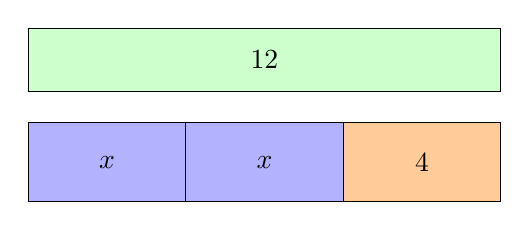
\begin{tikzpicture}
  \draw[fill=blue!30] (0,0) rectangle (2,1) node[midway] {$x$};
  \draw[fill=blue!30] (2,0) rectangle (4,1) node[midway] {$x$};
  \draw[fill=orange!40] (4,0) rectangle (6,1) node[midway] {$4$};
  \draw[fill=green!20] (0,1.4) rectangle (6,2.2) node[midway] {$12$};
\end{tikzpicture}
\end{center}

\begin{itemize}
  \item Write an equation represented by the bar model and solve it.
  \item If the total was 18 instead of 12, what would $x$ be?
  \item Is $3(x+4)=3x+4$ true or false? Explain.
\end{itemize}

\end{frame}

%------------------------------------------------
\begin{frame}{Starter 2}

\begin{itemize}
  \item Calculate: $6-11$
  \item Collect like terms: $5x + 2 + 3x$
  \item Expand: $4(a + 2)$
  \item Solve: $2x = 14$
\end{itemize}

\vspace{0.3cm}

\begin{center}
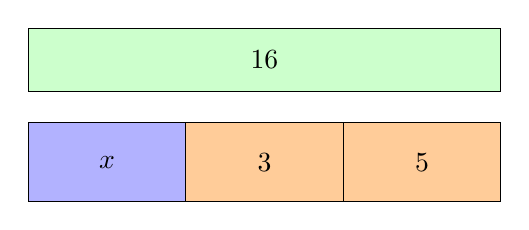
\begin{tikzpicture}
  \draw[fill=blue!30] (0,0) rectangle (2,1) node[midway] {$x$};
  \draw[fill=orange!40] (2,0) rectangle (4,1) node[midway] {$3$};
  \draw[fill=orange!40] (4,0) rectangle (6,1) node[midway] {$5$};
  \draw[fill=green!20] (0,1.4) rectangle (6,2.2) node[midway] {$16$};
\end{tikzpicture}
\end{center}

\begin{itemize}
  \item Write the equation represented by the bar model and solve it.
  \item Which part of the diagram represents the constant?
  \item Create a bar model for $8x + 2 = 26$.
  \item Simplify: $ax + bx$
\end{itemize}

\end{frame}

%------------------------------------------------
\begin{frame}{Starter 3}

\begin{itemize}
  \item Calculate: $-3 + 8$
  \item Collect like terms: $6a + 3 + 2a$
  \item Expand: $2(x + 7)$
  \item Solve: $x - 4 = 9$
\end{itemize}

\vspace{0.3cm}

\begin{center}
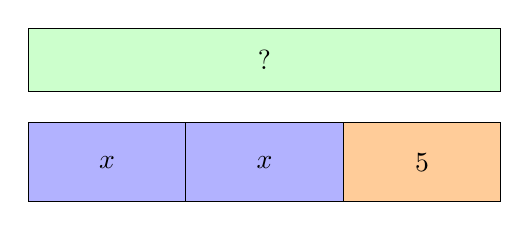
\begin{tikzpicture}
  \draw[fill=blue!30] (0,0) rectangle (2,1) node[midway] {$x$};
  \draw[fill=blue!30] (2,0) rectangle (4,1) node[midway] {$x$};
  \draw[fill=orange!40] (4,0) rectangle (6,1) node[midway] {$5$};
  \draw[fill=green!20] (0,1.4) rectangle (6,2.2) node[midway] {$?$};
\end{tikzpicture}
\end{center}

\begin{itemize}
  \item Suppose the total is 17. Write and solve the equation.
  \item Suppose the total is 25. What is $x$ now?
  \item Expand: $3(x+7)$
  \item Expand: $3(x-7)$
\end{itemize}

\end{frame}

%------------------------------------------------
\begin{frame}{Starter 4}

\begin{itemize}
  \item Calculate: $-6 \div 3$
  \item Collect like terms: $9a - 4a + 2 + 3b$
  \item Expand: $5(y + 3)$
  \item Solve: $3d = 18$
\end{itemize}

\vspace{0.3cm}

\begin{center}
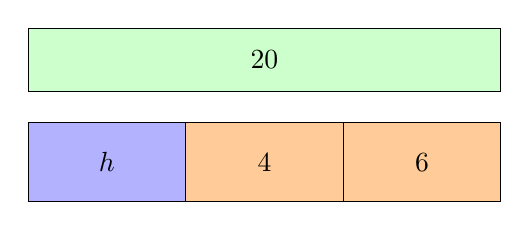
\begin{tikzpicture}
  \draw[fill=blue!30] (0,0) rectangle (2,1) node[midway] {$h$};
  \draw[fill=orange!40] (2,0) rectangle (4,1) node[midway] {$4$};
  \draw[fill=orange!40] (4,0) rectangle (6,1) node[midway] {$6$};
  \draw[fill=green!20] (0,1.4) rectangle (6,2.2) node[midway] {$20$};
\end{tikzpicture}
\end{center}

\begin{itemize}
  \item Write an equation represented by the diagram and solve for $h$.
  \item If the $4$ block was instead $h$ and the $h$ block was $4$, what equation would we have?
  \item Expand: $(x-3)(x-2)$
  \item Simplify: $a^2 \times a \times b$
\end{itemize}

\end{frame}

%------------------------------------------------
\begin{frame}{Starter 5}

\begin{itemize}
  \item Calculate: $7 - 12$
  \item Collect like terms: $2x + 7 + 3x$
  \item Expand: $3(a + 5)$
  \item Solve: $2x + 3 = 11$
\end{itemize}

\vspace{0.3cm}

\begin{center}
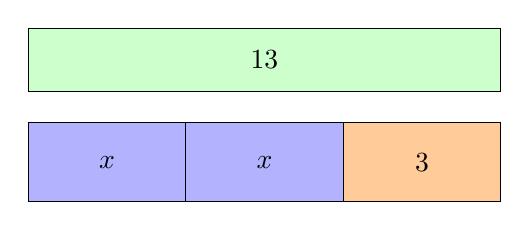
\begin{tikzpicture}
  \draw[fill=blue!30] (0,0) rectangle (2,1) node[midway] {$x$};
  \draw[fill=blue!30] (2,0) rectangle (4,1) node[midway] {$x$};
  \draw[fill=orange!40] (4,0) rectangle (6,1) node[midway] {$3$};
  \draw[fill=green!20] (0,1.4) rectangle (6,2.2) node[midway] {$13$};
\end{tikzpicture}
\end{center}

\begin{itemize}
  \item Write and solve the equation represented by the model.
  \item Explain how each part of the diagram matches the equation.
  \item Draw a bar model to represent $3x + 3 = 13$.
  \item Write an equation with solution $x=5$.
\end{itemize}

\end{frame}

%------------------------------------------------
\begin{frame}{Starter 6}

\begin{itemize}
  \item Calculate: $-4 \times 6$
  \item Collect like terms: $7x + 3x - 5$
  \item Expand: $2(3x + 4)$
  \item Solve: $3x + 5 = 17$
\end{itemize}

\vspace{0.2cm}

\begin{itemize}
  \item Solve: $4x + 3 = 2x + 15$
  \item Solve: $\frac{x}{3} + 4 = 9$
\end{itemize}

\vspace{0.3cm}

\begin{center}
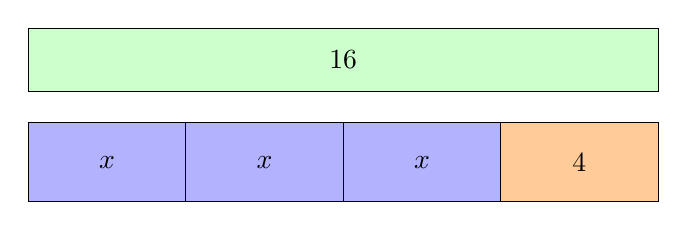
\begin{tikzpicture}

  \draw[fill=blue!30] (0,0) rectangle (2,1) node[midway] {$x$};
  \draw[fill=blue!30] (2,0) rectangle (4,1) node[midway] {$x$};
  \draw[fill=blue!30] (4,0) rectangle (6,1) node[midway] {$x$};
  \draw[fill=orange!40] (6,0) rectangle (8,1) node[midway] {$4$};
  \draw[fill=green!20] (0,1.4) rectangle (8,2.2) node[midway] {$16$};

\end{tikzpicture}
\end{center}

\begin{itemize}
  \item Write one equation that could be represented by this bar model.
  \item Write a different equation with the same solution.
  \item Create an equation with solution $x=4$ that includes a negative term.
\end{itemize}

\end{frame}

%------------------------------------------------

\end{document}